%
% $Id: chapter3.tex 3915 2009-06-18 13:28:32Z sliske $
%
%%\pagestyle{scrheadings}
%%\ohead[]{}
%%\ihead[]{}
%%\chead[]{}
%%\ofoot[\pagemark]{\pagemark}
%%\ifoot[]{}
\chapter{Design \& Implementation}
\label{sec:design}

\section{Requirements}

\section{Abstract Architecture}

\begin{figure}[p]
    \caption[IPC Architecture]{Abstract \ac{IPC} architecture }
    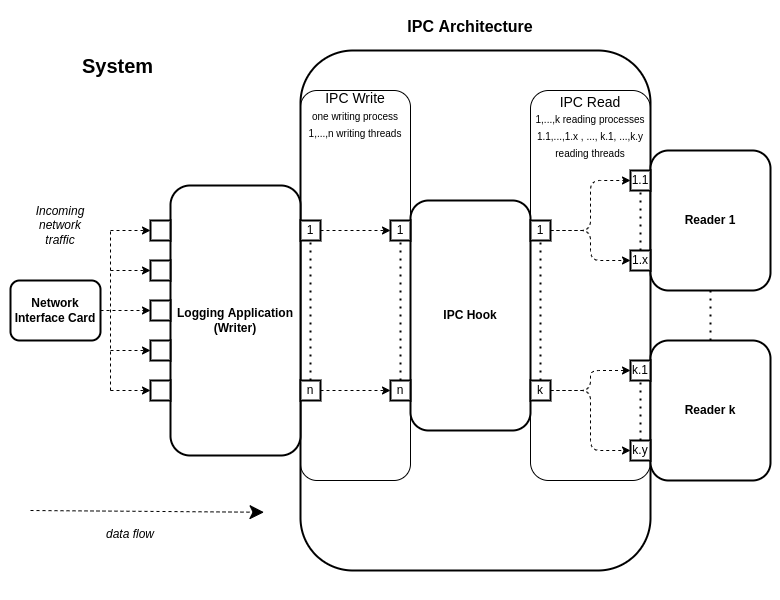
\includegraphics[width=\textwidth]{images/meta_ipc_architecture.png}
\end{figure}

\section{Choice of IPC Type}

\section{Shared Memory API}

\begin{figure}[p]
    \includegraphics[width=\textwidth]{images/shm_architecture.png}
    \caption[Shared Memory Architecture]{Architecture for the single-writer multi-reader shared memory ringbuffer for the transmission
    of log messages. }
\end{figure}

\section{Proof-of-Concept IPS}

\begin{figure}[p]
    \includegraphics[width=\textwidth]{images/ips_architecture.png}
    \caption[Simplefail2ban Architecture]{Activity diagram for the proof-of-concept IPS implementation. A variable number of ``banning threads'' receive log messages from a host and
    parse them with a predefined regular expressions. For messages that match the expression, the clients IP address is extracted from the log message and added to a hashtable, that keeps count of
    the number of matches per address. If the count reaches the configured limit, the address is added to the list of banned addresses with a current timestamp and inserted into the eBPF map. One ``unbanning
   thread'' routinely iterates through the banned list and checks, if a clients bantime hast elapsed. Clients with an elapsed bantime are removed from the eBPF map, banned list and hashtable.}
   \label{fig:meta_architecture}
\end{figure}

\section{Test Application}


